\documentclass{beamer}
% Heterogêneo +/-
% Grafo de possíveis sentenças
% Gráfico com as melhores
% Aquisição de dados
% - Reconhecida igual a correta
% - Reconhecida diferente da correta
% Geração do ARFF (pegar do proposta.tex)
% Rede neural dados empíricos
% Rescore
% Resultados


% This file is a solution template for:

% - Talk at a conference/colloquium.
% - Talk length is about 20min.
% - Style is ornate.

% Copyright 2004 by Till Tantau <tantau@users.sourceforge.net>.
%
% In principle, this file can be redistributed and/or modified under
% the terms of the GNU Public License, version 2.
%
% However, this file is supposed to be a template to be modified
% for your own needs. For this reason, if you use this file as a
% template and not specifically distribute it as part of a another
% package/program, I grant the extra permission to freely copy and
% modify this file as you see fit and even to delete this copyright
% notice.

%%%%%%%%%%% OPTIONS THAT ARE VALID FOR BOTH HANDOUTS AND NORMAL SLIDES %%%%%%%%
%\usepackage{beamerthemesplit}
\setbeamertemplate{footline}[frame number] % numerar slides
\setbeamertemplate{navigation symbols}{} % retirar barra de navegação

%%%%%%%%%%% OPTIONS THAT ARE VALID FOR NORMAL SLIDES %%%%%%%%
%AK: It seems I do not need it:
%\usepackage{pgfpages}
%\pgfpagesuselayout{resize}[a4paper,border shrink=5mm,landscape]
\mode<presentation> {\usetheme{Singapore}
\setbeamercovered{transparent}}
%\mode<presentation> {\usetheme{warsaw} }

\usepackage[english]{babel}
\usepackage[utf8]{inputenc}
%\usepackage[table]{xcolor}
\usepackage{color}
\usepackage{booktabs}

\graphicspath{{./figuras/}}

\usepackage{times}
\usepackage[T1]{fontenc}

\title[Lattice Rescore] % (optional, use only with long paper titles)
{Detecção e Correção de Confusão entre Fonemas em Reconhecimento Continuo de Voz}

\author%[]  (optional, for multiple authors)
{Pedro~Batista}%\inst{1}}
\institute % (optional)
{
Mineração de Dados\\
Programa de Pós-Graduação em Engenharia Elétrica - PPGEE \\
Universidade Federal do Pará - UFPA \\
http://www.laps.ufpa.br/pedro
}
% - Use the \inst command only if there are several affiliations.
% - Keep it simple, no one is interested in your street address.

\date[27 de Setembro de 2010] % (optional)
{Trabalho de Conclusão de Disciplina (Mineração de Dados)}

\subject{Reconhecimento Automático de Voz}

%\pgfdeclareimage[height=0.5cm]{university-logo}{../../latex/common_images/logo_broffice}
%\logo{\pgfuseimage{university-logo}}
% Delete this, if you do not want the table of contents to pop up at
% the beginning of each subsection:
\AtBeginSection[]
{
  \begin{frame}<beamer>{Sumário}
     \tableofcontents[currentsection]
     \end{frame}
}


% If you wish to uncover everything in a step-wise fashion, uncomment
% the following command:
%\beamerdefaultoverlayspecification{<+->}

\begin{document}

\begin{frame}
  \titlepage
\end{frame}

\begin{frame}{Sumário}

  \tableofcontents
  % You might wish to add the option [pausesections]
  \end{frame}
  % Structuring a talk is a difficult task and the following structure
  % may not be suitable. Here are some rules that apply for this
  % solution:

  % - Exactly two or three sections (other than the summary).
  % - At *most* three subsections per section.
  % - Talk about 30s to 2min per frame. So there should be between about
  %   15 and 30 frames, all told.

  % - A conference audience is likely to know very little of what you
  %   are going to talk about. So *simplify*!
  % - In a 20min talk, getting the main ideas across is hard
  %   enough. Leave out details, even if it means being less precise than
  %   you think necessary.
  % - If you omit details that are vital to the proof/implementation,
  %   just say so once. Everybody will be happy with that.

  \section{Introdução}
  \subsection{Definição}
  \frame{
  \begin{itemize}
    \item Reconhecimento Automático de Voz (RAV) e Síntese de Voz (TTS).
      \vspace{0.5cm}
      \includegraphics[height=3cm]{SintetizadorReconhecedor}
  \end{itemize}
  }

  %  \begin{frame}
  %    \frametitle{Por que Reconhecimento Automático de Voz?}
  %    \vspace{0.5cm}
  %    \includegraphics[height=3cm]{voice-controlled_car2}
  %    \hspace{1cm}
  %    \includegraphics[height=3cm]{voice-controlled_car}\\
  %
  %    \includegraphics[height=3cm]{voice-controlled_phone}
  %    \includegraphics[height=4.5cm]{speech_controlled_robotic-arm}
  %  \end{frame}

  \subsection{Como Funciona?}
  \frame{
  \frametitle{Como Funciona Reconhecimento Automático de Voz?}
  \begin{itemize}
    \item A fala é uma sequencia de palavras.
    \item Cada palavra consiste em uma série de sons (fonemas).
      {\centering \Large \texttt{noticia ->  n o tS i s i a}\\}
      \hspace{40pt} (grafema) \hspace{65pt} (fonema)\\[5pt]
      \pause
    \item Modelos estatísticos baseados em probabilidades:
      \begin{itemize}
	\item Acústica: cadeias escondidas de Markov (HMM).
	\item Da língua: modelos n-gramas.
      \end{itemize}
    \item Modelos não-probabilisticos: gramáticas livre de contexto.
  \end{itemize}
  }

  \frame{
  \frametitle{Processo de Reconhecimento}
  \begin{center}
    \includegraphics[height=1.4in]{diagrama_reconhecimento}
  \end{center}
  }

  \begin{frame}
    \frametitle{Aprendizado com o Resultado do Sistema}
    \begin{itemize}
      \item Melhorar o reconhecimento adicionando informação complementar.
      \item Encontrar padrões de erros.
      \item HMM é amplamente pesquisada / utilizada.
    \end{itemize}
  \end{frame}

  %TODO marcar as hipóteses
  \begin{frame}
    \frametitle{Saída do Reconhecedor (Lattice)}
    \only<1>{
    \begin{figure}[ht]
      \begin{center}
	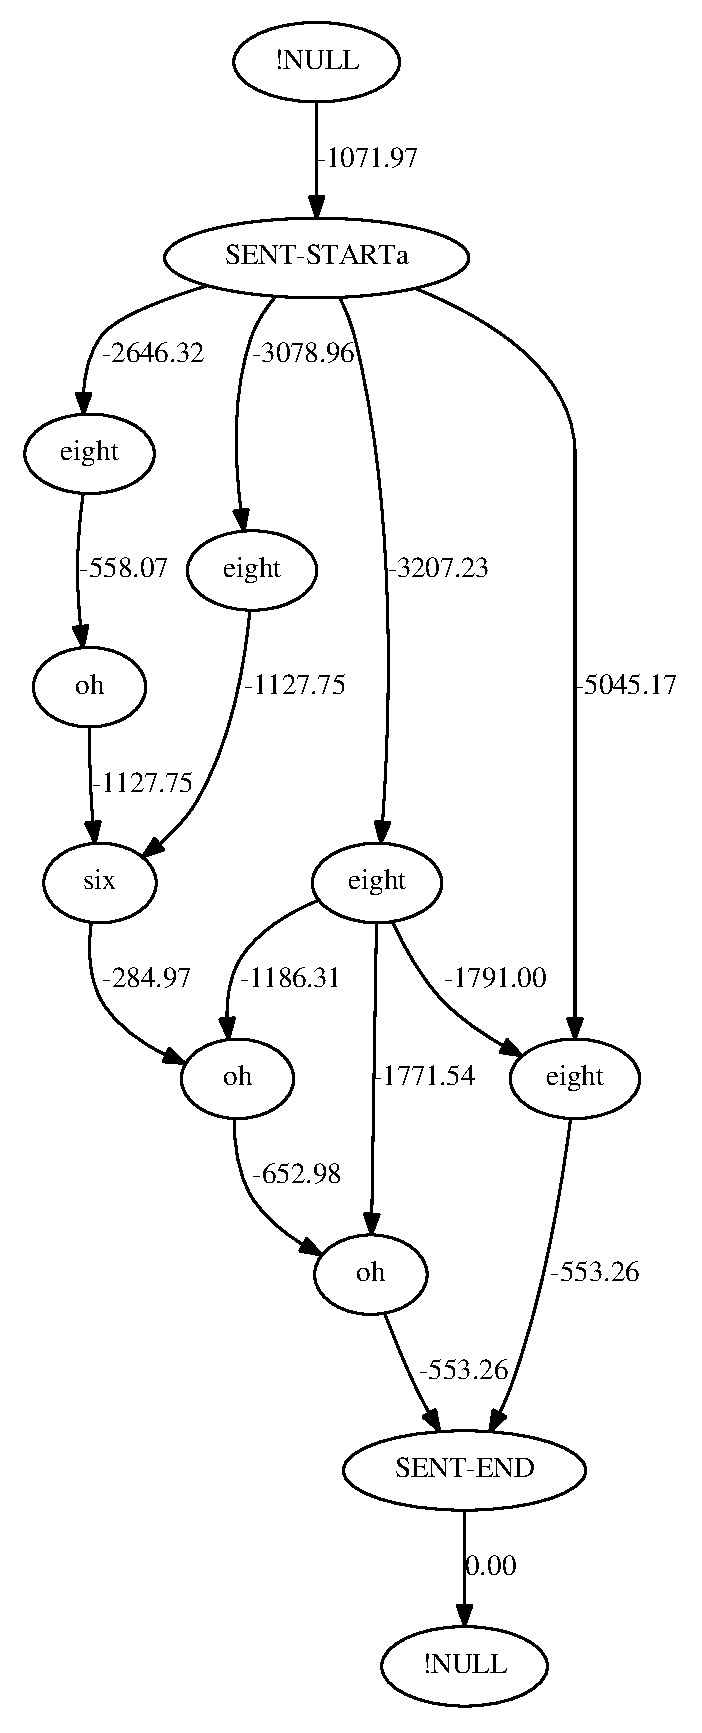
\includegraphics[width=1.2in]{lattice}
      \end{center}
      \caption{Exemplo de grafo (lattice) gerado pelo decodificador}
    \end{figure}}

    \only<2>{
    \begin{figure}[ht]
      \begin{center}
	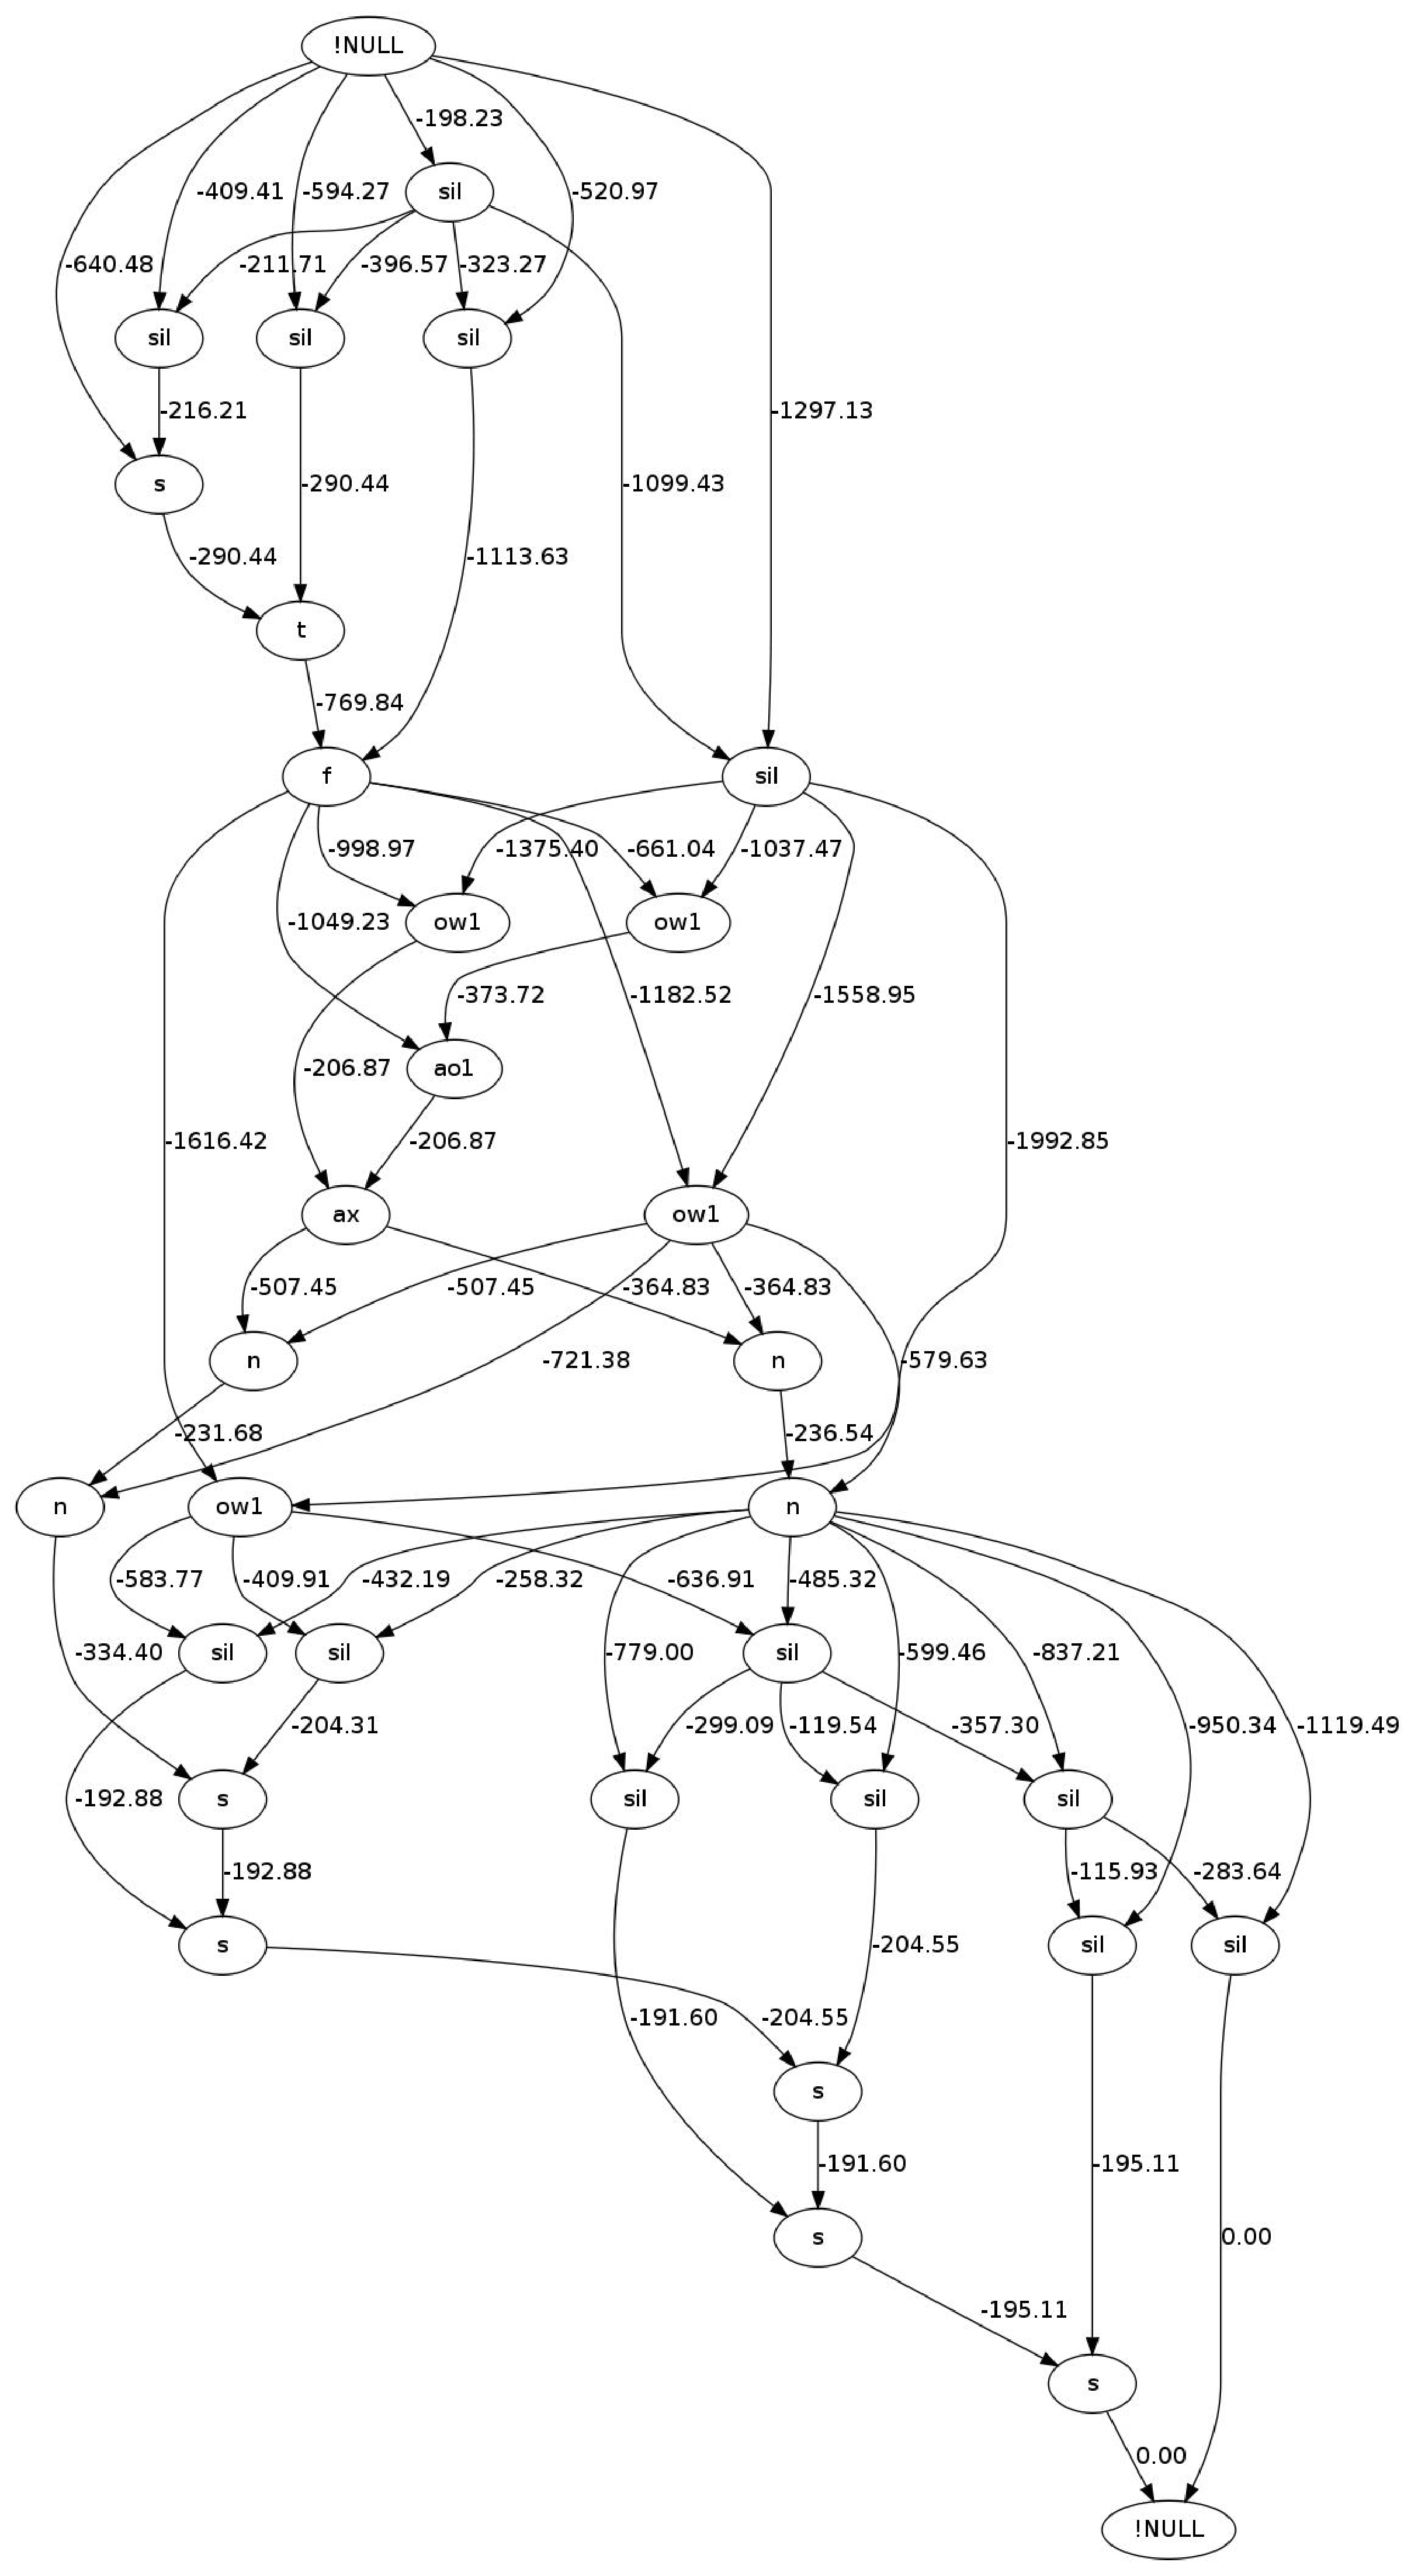
\includegraphics[width=1.7in]{jeao}
      \end{center}
      \caption{Exemplo de grafo (lattice) gerado pelo decodificador}
    \end{figure}}
  \end{frame}

  \begin{frame}
    \frametitle{Saída do Reconhecedor Melhores Sentenças}
    \begin{center}
      \vspace{0.1in}
      Margem
      $M(t) = b_{q^{*}_{i}}^{f_{s}}(t) - b_{q_{i}}^{f_{s}}(t)$
      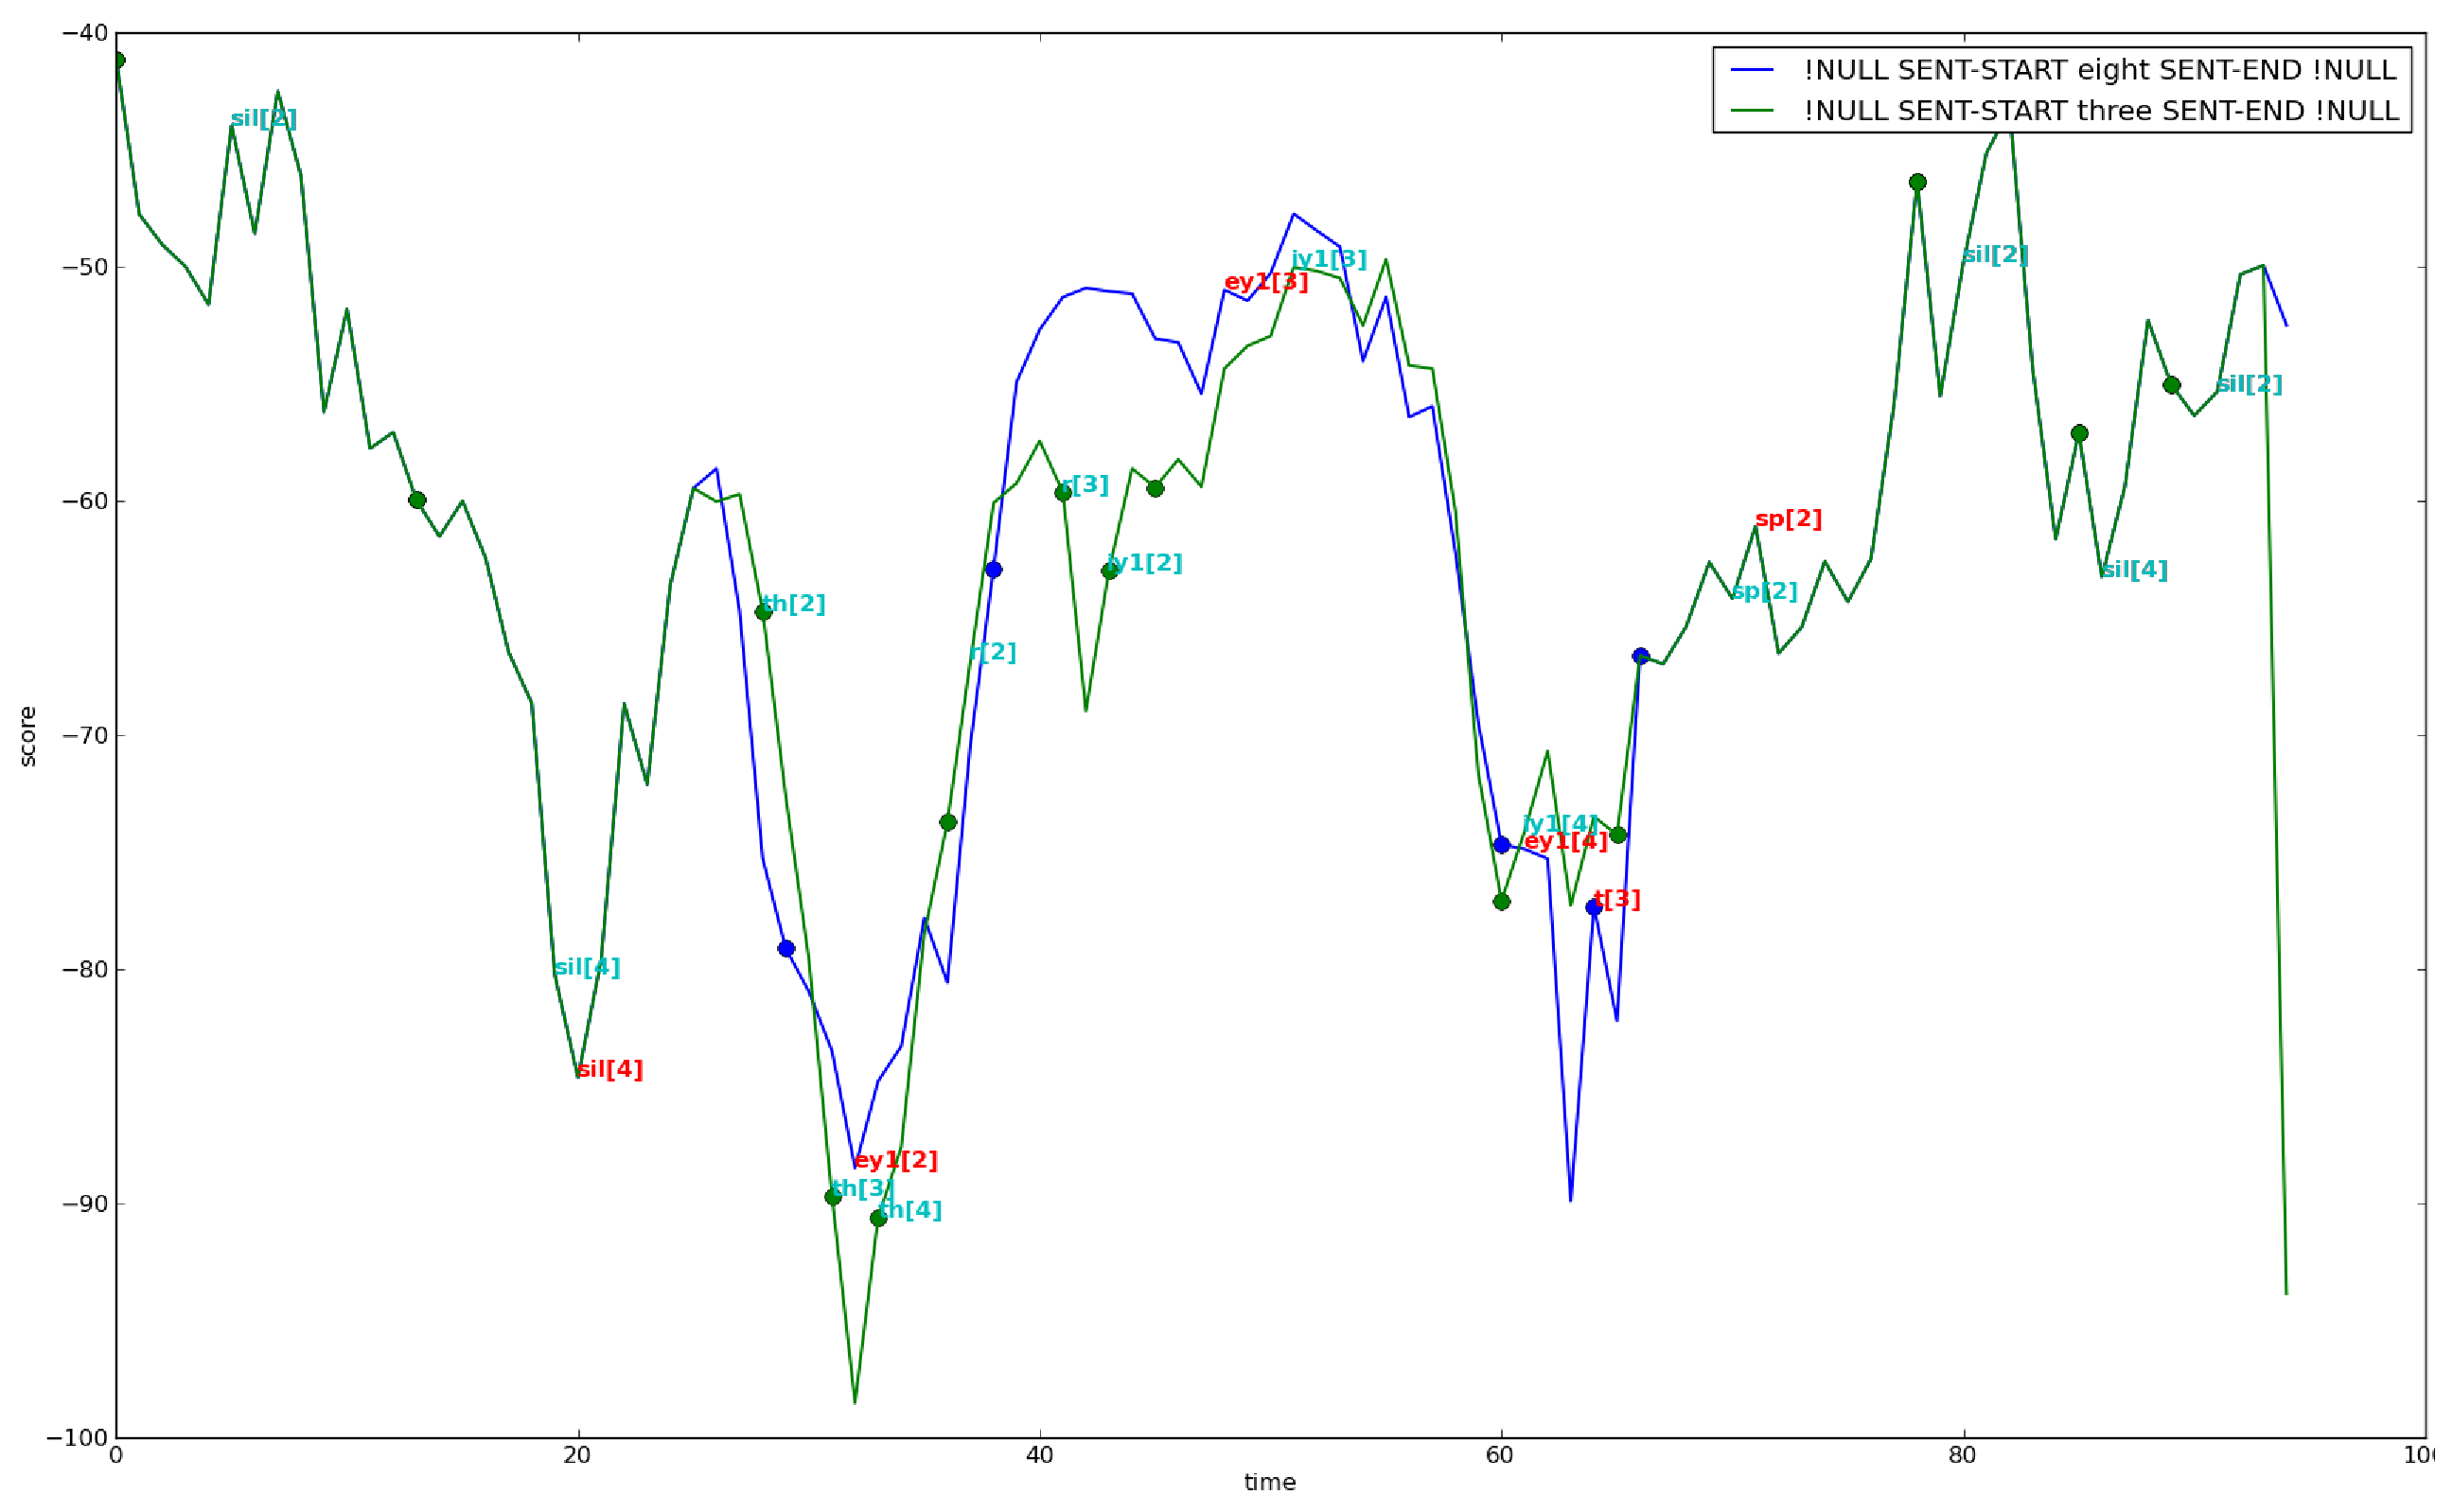
\includegraphics[width=4.6in]{9}
    \end{center}
  \end{frame}

  \section{Aquisição de Dados}
  \subsection{Onde está a Informação}
  \begin{frame}
    \frametitle{Reconhecida Diferente da Correta}
    \begin{figure}[ht]
      \begin{center}
	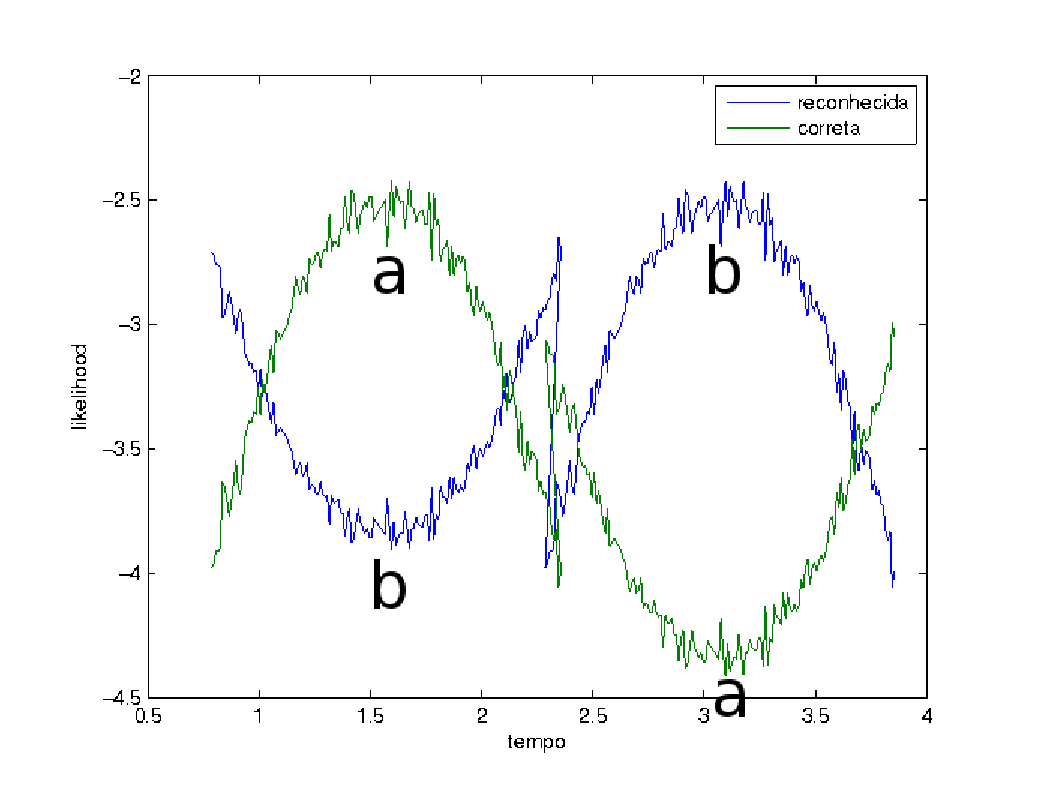
\includegraphics[width=2.5in]{corr_neq_rec}
      \end{center}
    \end{figure}
    \only<2>{ \begin{itemize}
      \item Quando $b > a$ temos uma confusão, pois $a$ deveria ganhar.
    \end{itemize}}
  \end{frame}

  \begin{frame}
    \frametitle{Reconhecida Igual a Correta}
    \begin{figure}[ht]
      \begin{center}
	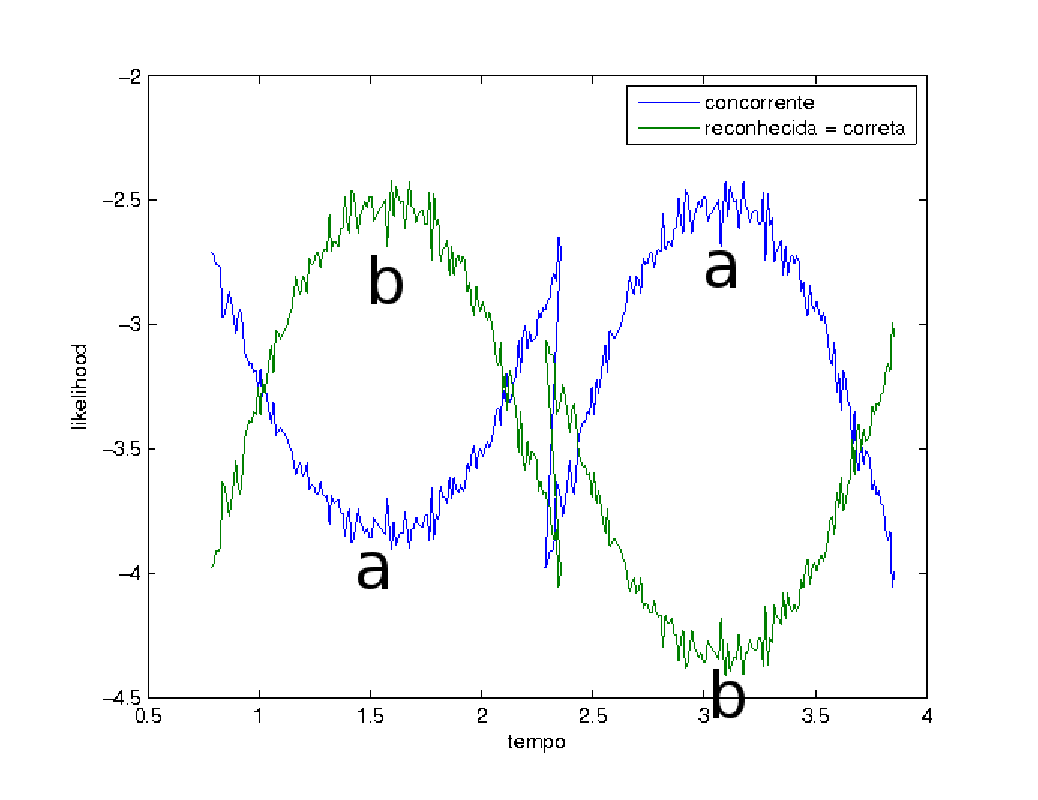
\includegraphics[width=2.5in]{corr_eq_rec}
      \end{center}
    \end{figure}
    \only<2>{\begin{itemize}
	\item Quando $b > a$ ao contrário do exemplo anterior não temos uma confusão, pois $b$ realmente deveria ganhar.
    \end{itemize}}
  \end{frame}

  \subsection{Busca por Novas Informações}
  \begin{frame}
    \frametitle{Os Dados não Foram Suficientes}
    \begin{itemize}
      \item O número de não confusões era muito superior ao número de confusões.
      \item Além disso devia-se dividir o conjunto em teste / validação e treino.
    \end{itemize}
  \end{frame}

  \begin{frame}
    \frametitle{Reconhecida Igual a Correta}
    \begin{figure}[ht]
      \begin{center}
	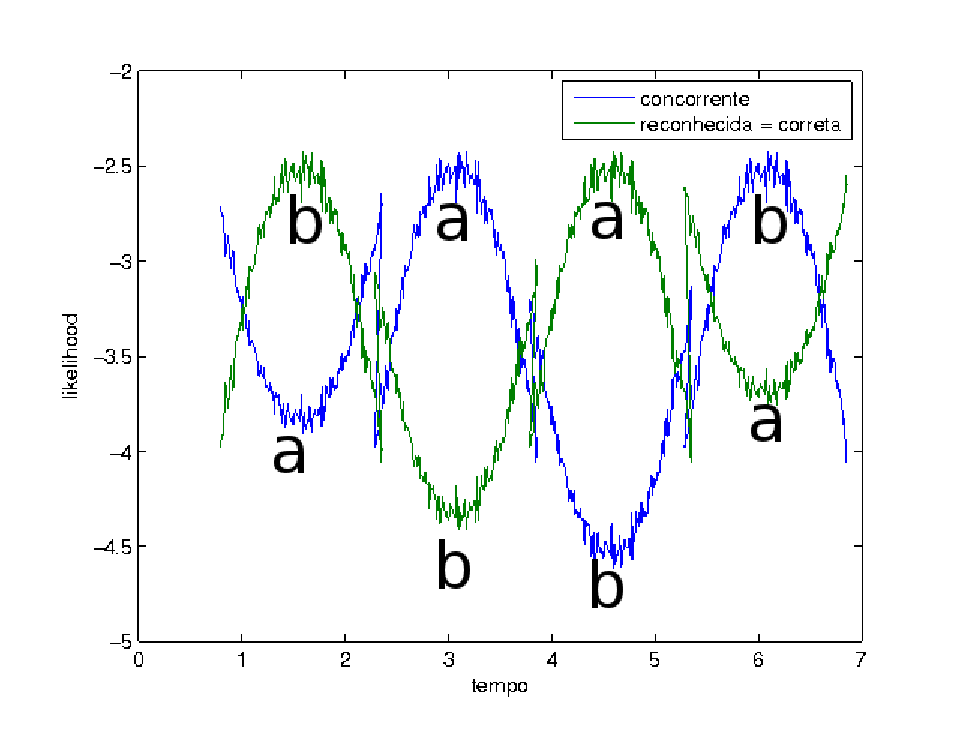
\includegraphics[width=2.5in]{corr_eq_rec_negative}
      \end{center}
    \end{figure}
    \only<2>{\begin{itemize}
	\item Observa-se que quando $b > a$, e $b$ está na sentença concorrente, $a$ deveria ganhar, além disso a margem nesse caso é negativa. Observa-se então um caso de confusão.
    \end{itemize}}
  \end{frame}

  \begin{frame}
    \frametitle{Quantidade de Dados}
    \begin{table}[!h]
      \centering
      \small
      %    \begin{tabular}{|p{2.8cm}|p{2.8cm}|p{2.8cm}|p{2.8cm}|}
      \begin{tabular}{|c|c|c|c|c|}
	\hline
	Maior score & Menor score & Confusuabilidade & Margem & Amostras \\
	\hline\hline
	%     $ah1_2$,$ah1_3$,$ah1_4$,$ow1_3$,$ow1_4$ & $uw1_4$ & no & positive \\
	$F^{'}_s\footnote{$F^{'}_s=\{ah1_2, ah1_3, ah1_4,ow1_3, ow1_4\}$}$ & $uw1_4$ & no & positive & 309 \\
	%     $uw1_4$ & $ah1_2, ah1_3, ah1_4, ow1_3, ow1_4$ & yes & negative \\
	$uw1_4$ & $F^{'}_s$ & yes & negative & 522 \\
	$ow1_2, ow1_3$ & $uw1_3$ & no & positive & 216 \\
	$uw1_3$ & $ow1_2, ow1_3$ & yes & negative & 682 \\
	$ow1_2$ & $uw1_2$ & no & positive & 14 \\
	$uw1_2$ & $ow1_2$ & yes & negative & 12 \\
	\hline
      \end{tabular}
    \end{table}
  \end{frame}

  \newcommand{\hnorm}{
  $\bar{H} = \begin{bmatrix}
    1& 1 &  1 &0.5(a) &0.88&0.94&1& 1 & 1(c) & 1
    \\ 1& 1 &0.83&0.86(c)&0.61&0.94&1&0.7& 0.55(e)& 1
    \\ 1&0.8&0.83& 1 (b) &  1 & 1  &1&0.5&  0.83 (d)& 1
    \\  ...&...&...&...&...&...&...&...&...&...  \end{bmatrix}$}

    \subsection{O Arquivo ARFF}
    \begin{frame}
      \frametitle{Montagem do Arquivo ARFF}
      \footnotesize
      \only<1>{
      \begin{itemize}
	\item As linhas da matriz H são hipóteses e as colunas frame.\\
      \end{itemize}
      $H = \begin{bmatrix}
	-80&-80&-100&-120(a)&-90&-80&-80&-50&-50(c)&-100
	\\ -80&-80&-120&-70(c)&-130&-80&-80&-70&-90(e)&-100
	\\ -80&-100&-120&-60(b)&-80&-75&-80&-100&-60(d)&-100
	\\  ...&...&...&...&...&...&...&...&...&... \end{bmatrix}$

	\begin{itemize}
	  \item A matriz $H$ é normalizada dividindo-se o $\arg \max_{q_i} b_{q_i}^{f_s}(t_i)$ pelo score acústico
	    $b_{q_i}^{f_s}(t_i)$
	\end{itemize}
	}

	\hnorm

	\begin{itemize}
	  \item Regiões de confusão, 3-5 (margem negativa), 8-9 (margem positiva).
	  \item Maiores margens, 4 e 9.
	\end{itemize}
	\only<2>{
	\begin{center}
	  {\large ARFF}\\[0.1in]
	  $\begin{matrix}
	    \text{a} & \text{b} & \text{c} & \text{d} & \text{e} & \text{confusão} \\
	    0.5 & 1 & 0.86 & 0 & 0 & sim \\
	    0  & 0 & 1 & 0.83 & 0.55 & não\\
	  \end{matrix}$
	\end{center}}
      \end{frame}

      \section{Resultados}
      \begin{frame}
	\frametitle{Tipos de Teste}
	\begin{itemize}
	  \item Somente as maiores margens são utilizadas (Validação).
	  \item Teste real com todas as sentenças.
	\end{itemize}
      \end{frame}

      \subsection{Validação}
      \begin{frame}
	\frametitle{Teste com as maiores margens (Validação)}
	\begin{table}
	  \centering
	  \begin{tabular}{c  c  c}
	    \toprule
	    Aquisição & Confusões & Não Confusões \\\midrule
	    Reconhecida = Correta & 795 & 426 \\
	    Reconhecida $\neq$ Correta & 30&  - \\\midrule
	    \multicolumn{3}{c}{Utilizadas}  \\\midrule
	    Treino & 795 & 411 \\
	    Teste & 30 & 15 \\\bottomrule
	  \end{tabular}
	\end{table}
	\pause
	\begin{itemize}
	  \item Variando parâmetros da Rede Neural, como quantidade de camadas, taxa de aprendizagem e conjunto de validação.
	  \item 87.5\% de acerto.
	\end{itemize}
      \end{frame}

      \subsection{Teste Real}
      \begin{frame}
	\frametitle{Testes com Sentenças Erradas}
	\begin{table}[!h]
	  \centering
	  \small
	  \begin{tabular}{c p{0.8in} p{0.8in} p{0.8in}}
	    \toprule
	    & Sentenças Corretas & Sentenças Erradas & Taxa de Erro \\\midrule
	    Antes do Rescore & 15 & 30 & 66.70\% \\
	    Depois do Rescore & 41  & 4 & 8.80\% \\
	    \bottomrule
	  \end{tabular}
	\end{table}
      \end{frame}

      \section{Conclusão}
      \subsection{Sistema Viável}
      \begin{frame}
	\frametitle{Conclusão}
	\begin{itemize}
	  \item O trabalho mostrou que é possível reconhecer padrões e corrigir os erros e reconhecimento.
	\end{itemize}\vspace{0.5in}
	\pause
	\textcolor{blue}{\large Trabalhos Futuros}
	\begin{itemize}
	  \item Melhorar a Rede Neural.
	  \item Fazer testes com mais de um fonema de confusão.
	  \item Fazer testes de WER (word error rate).
	  \item Implementar em um sistema maior.
	\end{itemize}
      \end{frame}
      \begin{frame}
	\large
	\frametitle{Obrigado! Perguntas?}
	\begin{figure}
	  \includegraphics[height=1in]{logo}\\
	  
\includegraphics[height=0.8in]{logo_ufpa}
	  \includegraphics[height=0.4in]{logo_laps}\\
	\end{figure}
      \end{frame}

      \end{document}
